% ==================================================================================================================================
% Introduction

Ici, nous nous intéressons à l'analyse des fonctions non périodiques sur $\R$. 
Nous allons étudier une fonctions permettant d'isoler les principales composantes d'une fonction non périodique. 
L'analogie habituelle est de comparer une fonction, ici dite non régulière, avec un signal, par exemple sonore. 

Un tel signal est composé de différentes fréquences. En effet, on peut le décomposer en différents signaux 
périodiques, dont chacun est responsable d'une fréquence précise du signal de départ. 
Une fois ce signal décomposé, on peut isoler les fréquences qui ne nous intéressent pas et effectuer l'opération inverse. 

On obtient alors un nouveau signal issu du signal de départ avec, par exemple, une suppression du bruit. 
Une telle application est appelée tranformée de Fourier. 

\section{Transformée de Fourier}

\subsection{Définition et propriétés}

\begin{definition}[Transformée de Fourier]
    Soit $f \in L^1(\R)$, on définit l'application :
        \[ \mathcal{F} : 
            \begin{cases}
                L^1 \longrightarrow \mathcal{C}_b \\
                f \longmapsto \hat{f} 
            \end{cases}
        \text{où} \quad 
        \hat{f} :
        \begin{cases}
            \R \longrightarrow \C \\
            \xi \mapsto \int e^{-2i\pi \xi x} f(x) \; dx 
        \end{cases}
        \]
    Ici, $\mathcal{F}$ est la fonction transformée de Fourier. $\mathcal{C}_b$ représente l'ensemble des fonctions continues bornées. 
\end{definition}

\begin{prop}[Transformée de Fourier]
    La fonction transformée de Fourier possède énormément de propriétés, en voici quelques unes :
    \begin{itemize}
        \item \underline{Lemme de Riemann-Lebesgue} :
            \[ \boxed{ \forall f \in L^1, \quad \hat{f} \in \mathcal{C}^0 } \]
       \item $\mathcal{F}$ est $\mathcal{C}^0$
       \item $\mathcal{F}$ est \textbf{injective}. 
       \item $\mathcal{F}$ transforme les convolutions en produit 
        \[ \boxed{ \text{i.e} \quad \forall f,g \in L^1, \; \hat{f} \ast \hat{g} = \hat{f} \hat{g} \iff \mathcal{F}(f \ast g) = \mathcal{F}(f) \times \mathcal{F}(g) }\] 
        \item $\mathcal{F}$ transforme les dérivations en produits par des polynômes : 
            \begin{align*}
                & \text{si } \quad f \in L^1 \cap C^1 \text{ telle que } f \in L^1 \\ 
                & \text{alors } \quad \widehat{f'} = M \hat{f} \text{ où } M : \xi \longrightarrow 2 \pi i \xi  
            \end{align*}
        \item \underline{Formule de symétrie} :
            \[ \forall f,g \in L^1, \quad \int f \hat{g} \; d \lambda = \int \hat{f} g \; d \lambda \] 
    \end{itemize}
\end{prop}

\subsection{Inverse de la tranformée de Fourier}

\begin{theorem}[Inversion]
        \[ \text{Posons } \mathcal{F} : 
            \begin{cases}
                L^1 \longrightarrow C^0  \\ 
                f \longmapsto \check{f} = R \circ \mathcal{F}(f)
            \end{cases}
        \] telle que $\overline{\mathcal{F}} = R \circ \mathcal{F}$
    où $R : f \longmapsto (\xi \mapsto f(-\xi))$. On a alors :
            \[ \boxed{ \check{f}(\xi) = \widehat{f}(-\xi) \int e^{+ 2i\pi x \xi } f(x) \; dx }\] 
    Soit $f \in L^1$ telle que $\hat{f} \in L^1$ on a alors : 
            \[  \forall x \in X, \; f(x) = \overline{\mathcal{F}}(\hat{f})(x) \text{ p.p} \]
            \[ \text{i.e } f = \check{\hat{f}} = \hat{\check{f}} \text{ p.p} \]
\end{theorem}

\begin{remark}
    $\overline{\mathcal{F}(f)} = \overline{\mathcal{F}}(\overline{f})$ où $\overline{f}$ est le conjugué de $f$. 
\end{remark}

\begin{corollary}[Théorème d'inversion]
    \begin{itemize}
        \item $\mathcal{F}$ est injective
        \item $\mathcal{F}_{ | \mathcal{F}^{-1}(L^1)}$ est une bijection de $\mathcal{F}^{-1}(L^1)$ vers $\mathcal{F}^{-1}(L^1)$. 
        On note alors $\mathcal{A} := \mathcal{F}^{-1}(L^1)$. 
    \end{itemize}
\end{corollary}

\subsection{Propriétés de la transformée de Fourier sur $\mathcal{A}$}

\begin{theorem}[Egalité de Plancherel]
    Soient $f,g \in \mathcal{A}$ telles que :
    \begin{align*}
        \langle f,g \rangle_{L^2} &= \langle \hat{f}, \hat{g} \rangle_{L^2} \\ 
        \text{i.e } & \int f \overline{g} \; d \lambda = \int \hat{f} \times \overline{\hat{g}} \; d \lambda \\ 
        \text{i.e } & \langle f, g \rangle_{L^2} = \langle \mathcal{F}(f), \mathcal{F}(g) \rangle_{L^2}
    \end{align*}

    Donc si $f=g$, alors $\| f \|_2 = \| \hat{f} \|_2$. 
    
    Donc $ \mathcal{F}$ est une \textbf{isométrie} linéaire bijective de $ \mathcal{A}$ vers $ \mathcal{A}$ pour $\|.\|_2$.
\end{theorem}

\begin{theorem}[Propriétés de $ \mathcal{F}$ sur $L^2$]
    $ \mathcal{F} : L^2 \longrightarrow L^2$ est une isométrie linéaire bijective et :
    \begin{itemize}
        \item $ \forall f, g \in L^2, \quad \langle f, g \rangle = \langle \hat{f} , \hat{g} \rangle$ 
        \item $ \forall f, g \in L^2, \quad \widehat{fg} = \hat{f} \ast \hat{g} $ 
    \end{itemize}
\end{theorem}

\begin{remark}
    Soit $ f \in L^2$ l'expression $$ \hat{f}(\xi) = \int e^{-2 \pi i x \xi} f(x) \; dx $$ n'a pas de sens a priori dans le cas où $f \in L^2 \backslash L^1$. 
    {Mais} on peut trouver une suite de fonction de $L^1 \cap L^2$ telle que $f$ en soit la limite et ainsi écrire $f$ comme une limite de fonctions de $L^1 \cap L^2$.
\end{remark}

\begin{example}[Transformée de Fourier et Gaussienne]

    \vspace{0.5cm}
    
    \begin{multicols}{2}
        \[ \gamma_a : 
            \begin{cases}
                \R \longrightarrow \R \\ 
                x \longmapsto e^{- \pi a x^2}
            \end{cases}
        \]
    
        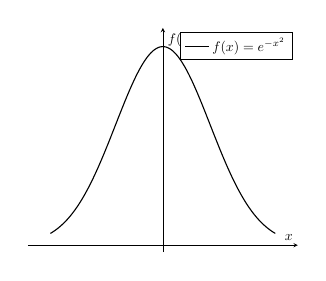
\begin{tikzpicture}[scale=0.5]
            \begin{axis}[
                axis lines=middle, % Place les axes au centre
                xlabel={$x$}, % Étiquette pour l'axe x
                ylabel={$f(x)$}, % Étiquette pour l'axe y
                domain=-30:30, % Intervalle de définition de la fonction
                samples=200, % Nombre de points pour tracer la courbe
                %grid=both, % Affiche la grille
                major grid style={line width=0.8pt,draw=gray!50}, % Style de la grille principale
                minor grid style={line width=0.4pt,draw=gray!20}, % Style de la grille secondaire
                enlargelimits=true, % Laisse un espace autour des données
                xtick=\empty, % Supprime les valeurs de l'axe x
                ytick=\empty, % Supprime les valeurs de l'axe y
                ]
                % Trace de la gaussienne
                \addplot[black, thick] {exp(-x^2*pi*0.001)};
                % Légende
                \addlegendentry{$f(x) = e^{-x^2}$}
            \end{axis}
        \end{tikzpicture}
    \end{multicols}

    Et en appliquant la transformée de Fourier, on obtient :

    \begin{multicols}{2}
        \[ \hat{\gamma}_a = a^{-1/2} \gamma_{\frac{1}{a}} \] 
        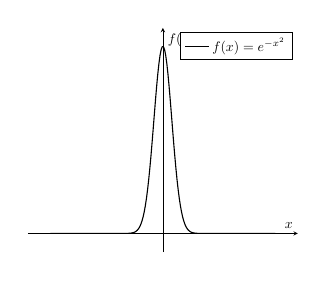
\begin{tikzpicture}[scale=0.5]
            \begin{axis}[
                axis lines=middle, % Place les axes au centre
                xlabel={$x$}, % Étiquette pour l'axe x
                ylabel={$f(x)$}, % Étiquette pour l'axe y
                domain=-5:5, % Intervalle de définition de la fonction
                samples=200, % Nombre de points pour tracer la courbe
                %grid=both, % Affiche la grille
                major grid style={line width=0.8pt,draw=gray!50}, % Style de la grille principale
                minor grid style={line width=0.4pt,draw=gray!20}, % Style de la grille secondaire
                enlargelimits=true, % Laisse un espace autour des données
                xtick=\empty, % Supprime les valeurs de l'axe x
                ytick=\empty, % Supprime les valeurs de l'axe y
                ]
                % Trace de la gaussienne
                \addplot[black, thick] {exp(-x^2*pi)};
                % Légende
                \addlegendentry{$f(x) = e^{-x^2}$}
            \end{axis}
        \end{tikzpicture}
    \end{multicols}
    
    Visuellement,la transformée de Fourier permet donc "d'isoler" les signaux d'une courbe. 
\end{example}